% !TEX root = main.tex
\section{Time dependent fit}
\label{sec:Tfit}

This section will cover the phasespace integrated, time dependent fit to $\Bs\to\Ds\hadron\pion\pion$ data, which is described by the PDF formulated in Eq. \ref{eq:PDF_intX}.
For the phasespace integrated fit to $\Bs\to\Ds\kaon\pion\pion$ data, the sensitivity to the CKM phase $\gamma$ will depend on the magnitude of the coherence factor $\kappa$, defined in Eq. \ref{eq:coherenceFactor}, 
which is added as an additional fit parameter. 
In order to avoid any pollution of the final data samples by background events, both samples are weighted using the sWeights obtained by the fits to the invariant mass distributions, described in Sec. \ref{sec: massfits}.
This fit approach is commonly known as \textit{sFit}. 
As additional input to the fit, the tagging information (Sec. \ref{sec:Tagging}), 
as well as the decay time acceptance (Sec. \ref{sec:Acceptance}) and resolution (Sec. \ref{sec:Resolution}) is used and fixed to the values obtained by the dedicated studies. 
Taking all inputs into account, the final time dependent fit PDF is given by

\begin{equation}
\label{eq:TPDF_full}
\mathcal{PDF}(t,\vec{\lambda}) = \left(\epsilon(t)\cdot \int P(x,t,q_t,q_f) \text d x \right) \times \mathcal{R}(t - t^{'}),
\end{equation}

where $\int P(x,t,q_t,q_f) \text d$ is the PDF given by Eq. \ref{eq:PDF_intX}, $\epsilon(t)$ is the efficiency due to the time acceptance effects and $\mathcal{R}(t - t^{'})$ is the Gaussian time resolution function. 



\subsection{sFit to $\Bs\to\Ds\pion\pion\pion$ data}  
The phasespace-integrated, time-dependent fit is performed to the full sWeighted sample of selected candidates from Run I and 2015+2016 Run II data, containing both possible magnet polarities and $\Ds$ final states.
In the fit, the values of $\Gs$ and $\DGs$ are fixed to the latest PDG report. All tagging parameters are fixed to the central values found in the tagging calibration, described in Sec. \ref{sec:Tagging}.
Due to the fact that the $\Bs\to\Ds\pion\pion\pion$ decay is flavour specific, the CP-coefficients can be fixed to $C=1$ and $D_{f} = D_{\bar{f}} = S_{f} = S_{\bar{f}} = 0$, reducing Eq. \ref{eq:PDF_intX} to

\begin{equation}
\int P(x,t,q_t,q_f) \text d x = [\text{cosh} \left( \frac{\Delta \Gamma \, t}{2}\right) + q_t q_f \, C \, \text{cos} \left( m_s \, t \right)] e^{- \Gamma t}.
\end{equation}

Note that in this case, the dependence on the coherence factor $\kappa$ is dropped and the same relation as found for $\Bs\to\Ds\pion$ decays is recovered. 
Therefore, the only free fit parameter left is $\dms$. The data distribution with the overlaid fit is shown in Fig. xXx and the obtained value for the mixing frequency is

\begin{equation}
\label{eq:dms_from_Norm}
\dms = xx.xxx \pm 0.yyy.
\end{equation}

\begin{figure}[h]
	\centering
		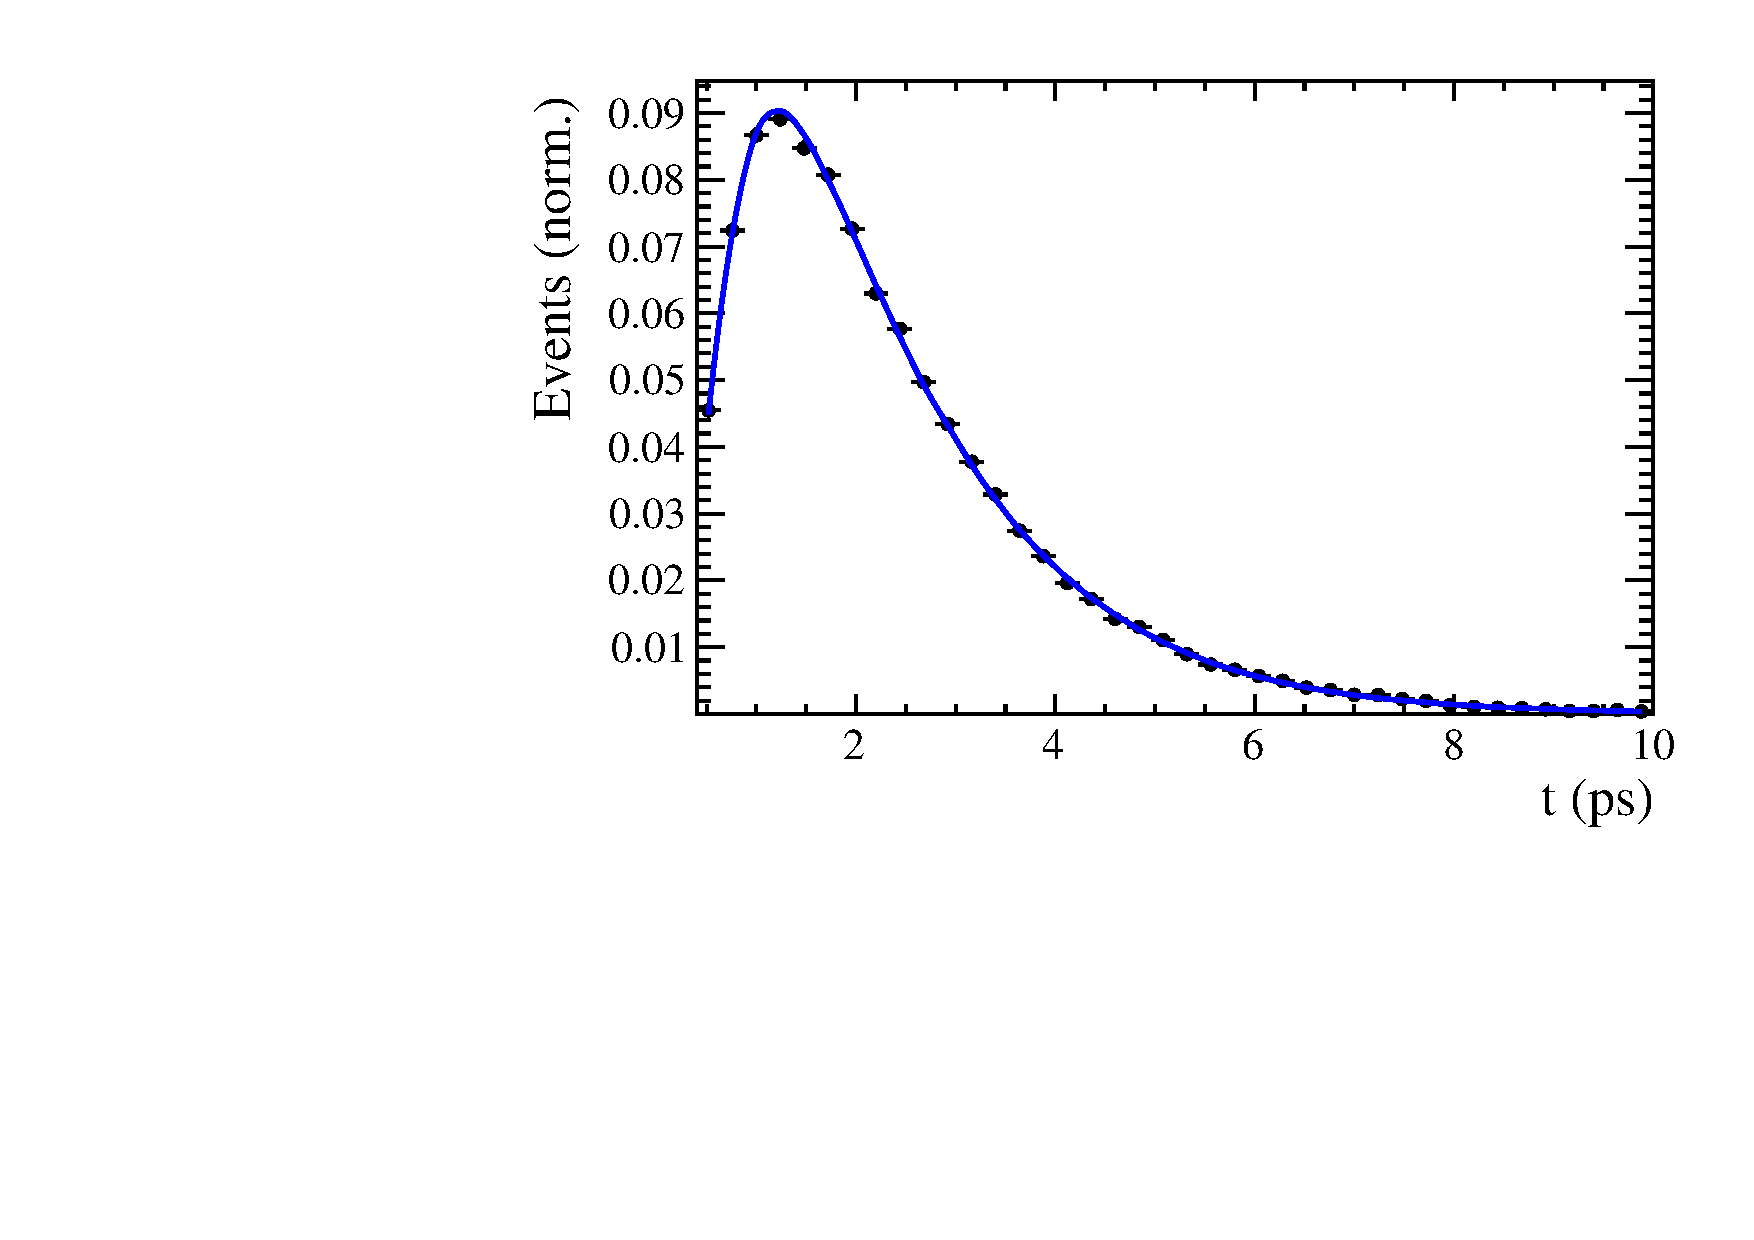
\includegraphics[width=0.45\textwidth, height = !]{figs/timeFit/norm_taggingCalib/h_t.pdf} 
		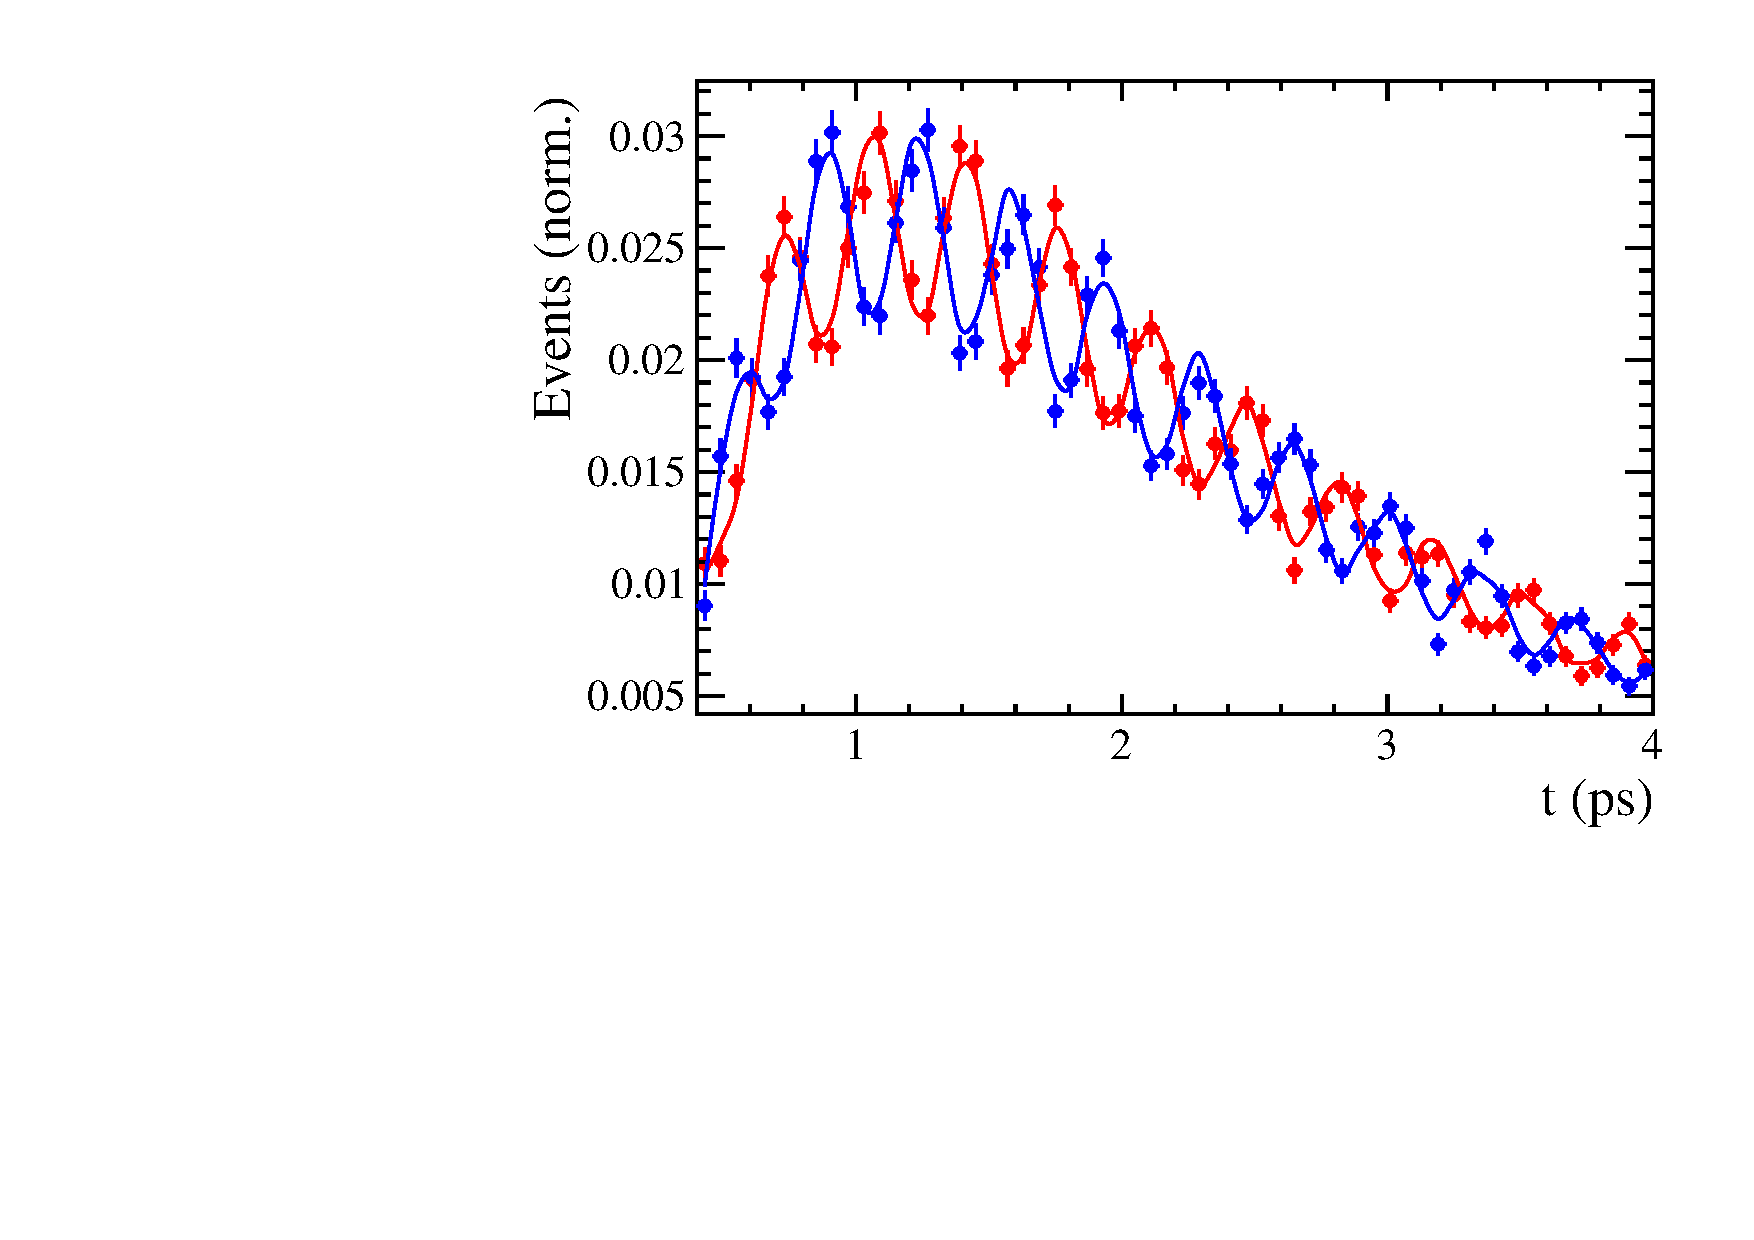
\includegraphics[width=0.45\textwidth, height = !]{figs/timeFit/norm_taggingCalib/h_t_mixed.pdf} 

		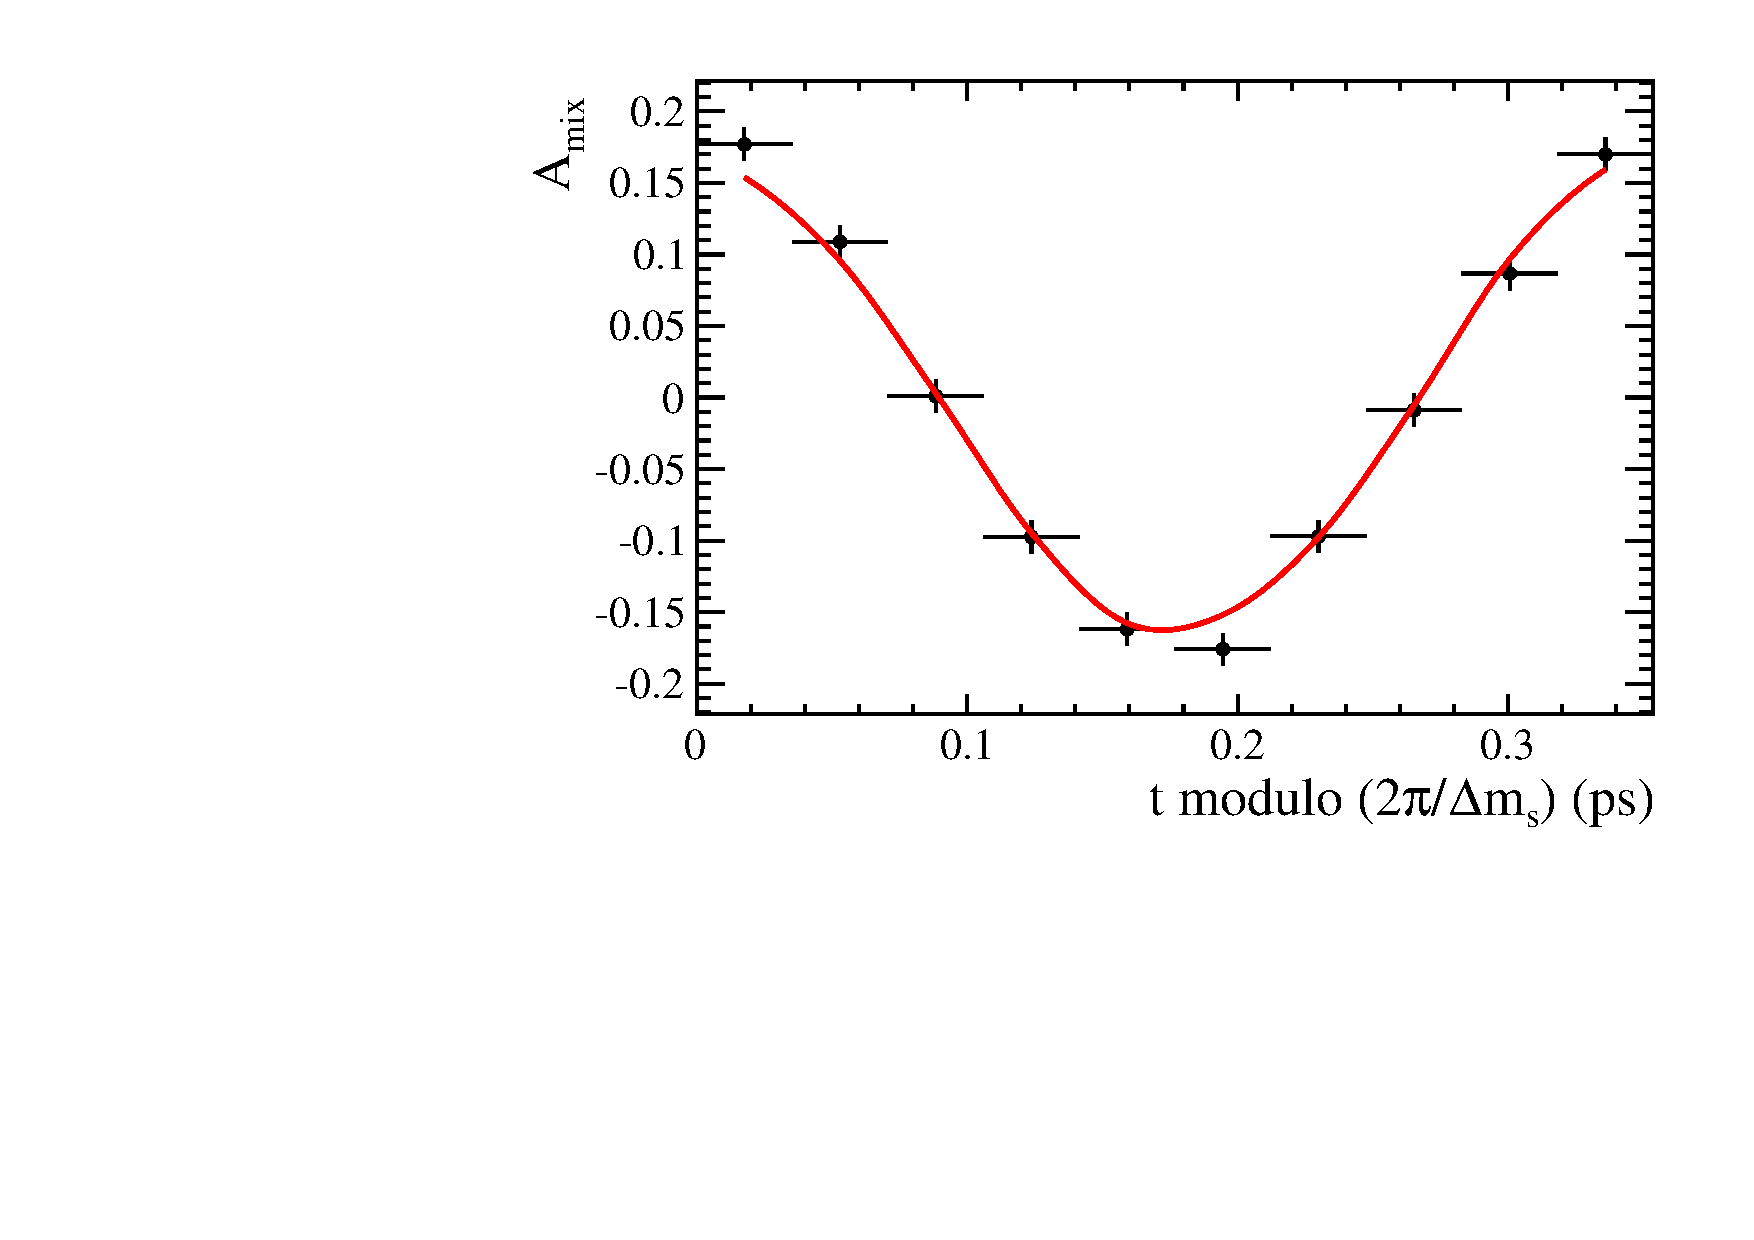
\includegraphics[width=0.45\textwidth, height = !]{figs/timeFit/norm_taggingCalib/h_asym.pdf} 		
		\caption{} 		
\end{figure}	

\subsection{sFit to $\Bs\to\Ds\kaon\pion\pion$ data}

\begin{figure}[h]
	\centering
		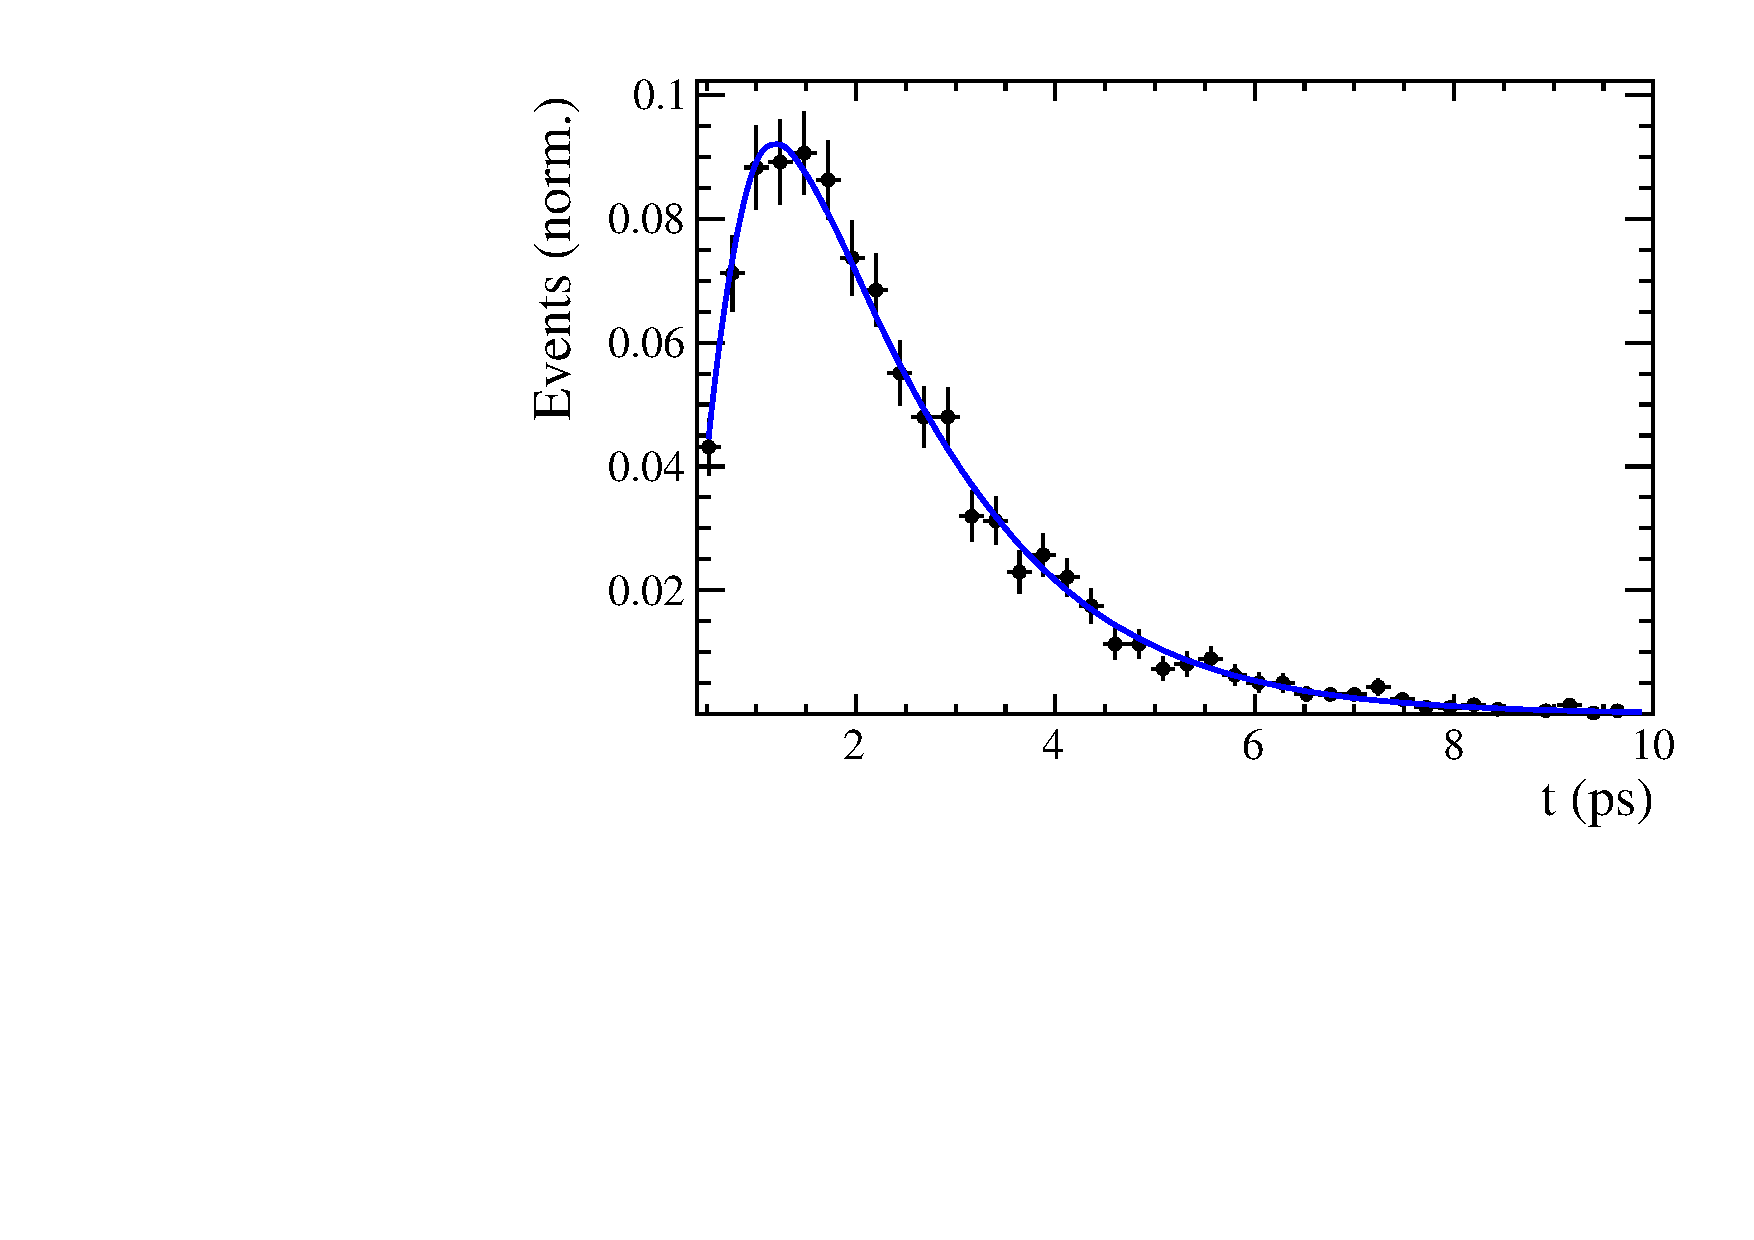
\includegraphics[width=0.45\textwidth, height = !]{figs/timeFit/signal/h_t.pdf} 
%		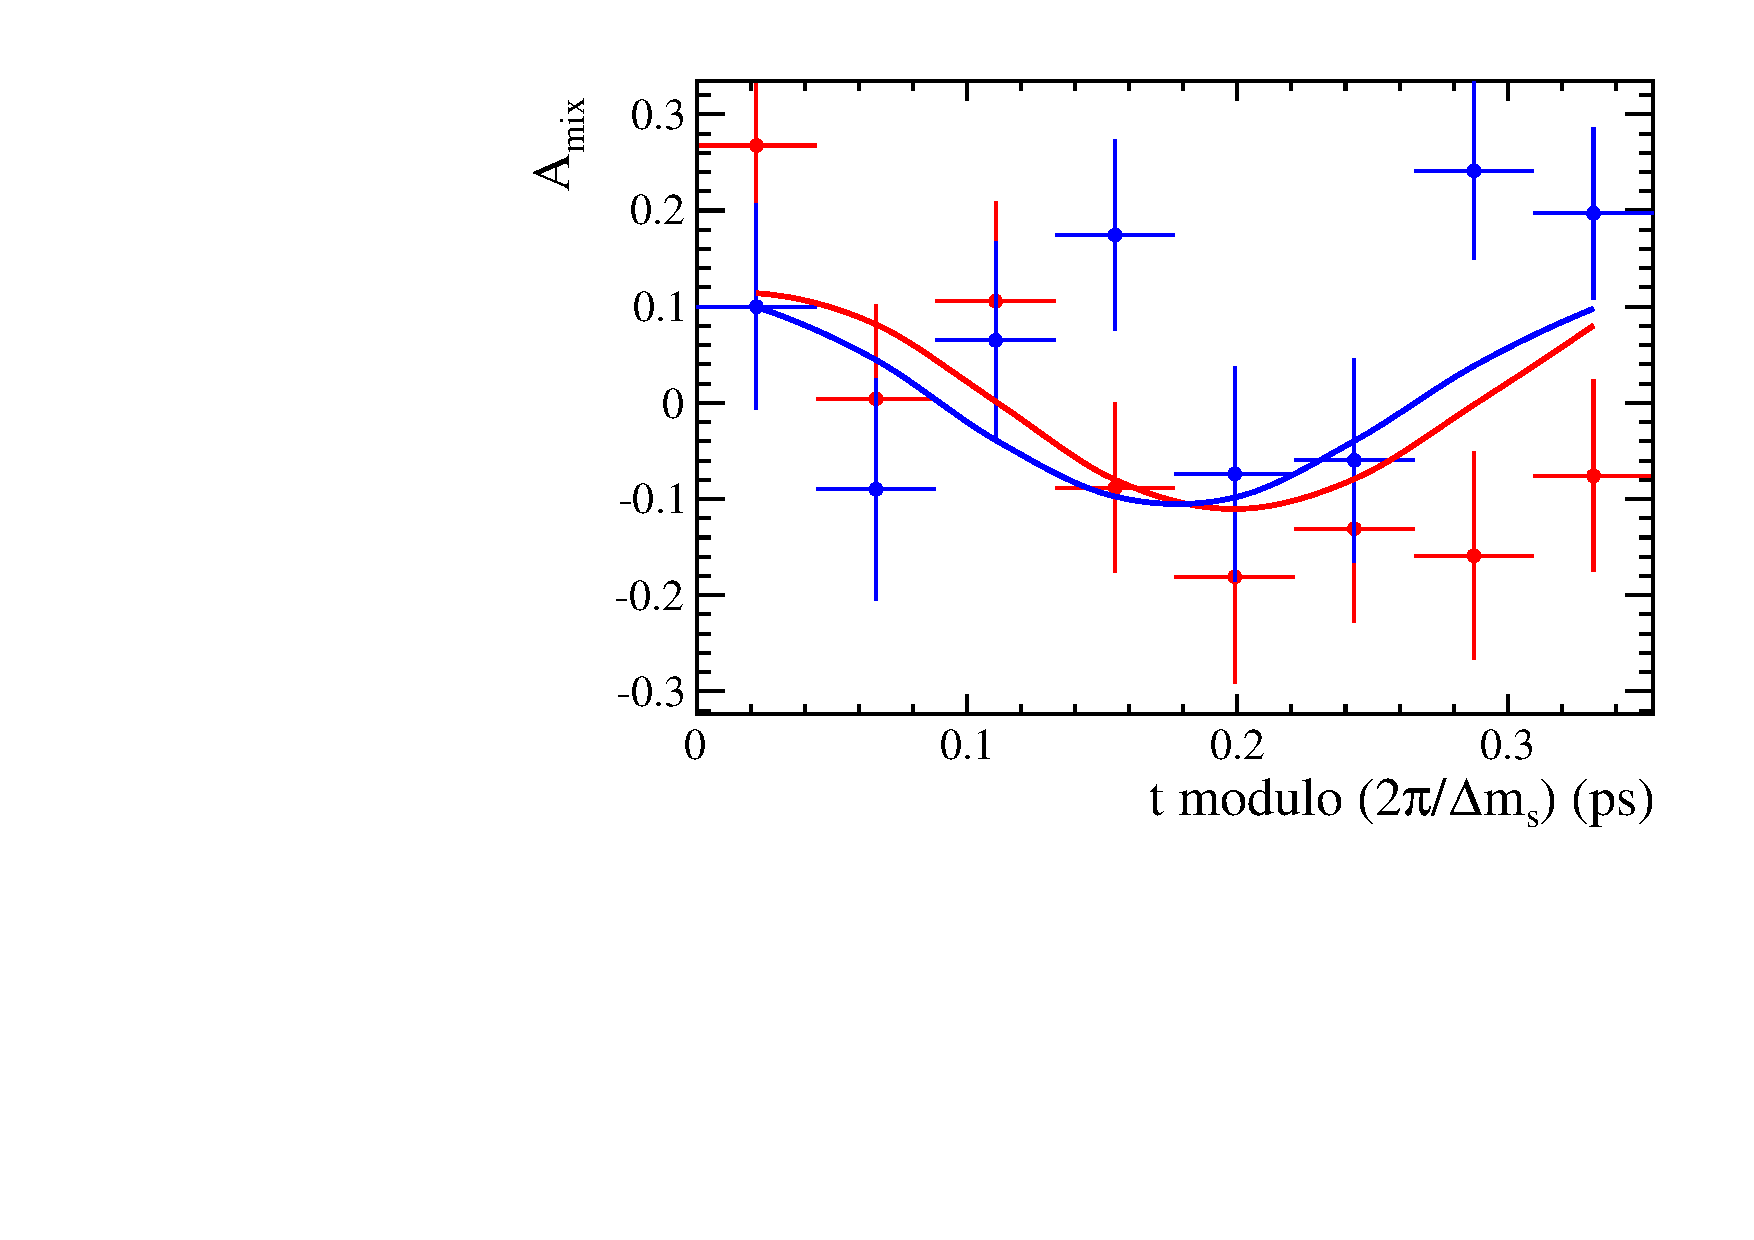
\includegraphics[width=0.45\textwidth, height = !]{figs/timeFit/signal/h_asym.pdf} 		
		\caption{} 		
\end{figure}	



%\subsection{Results}
